\subsection{Klassen-Diagramm}
	\begin{figure}[H]
        \centering
        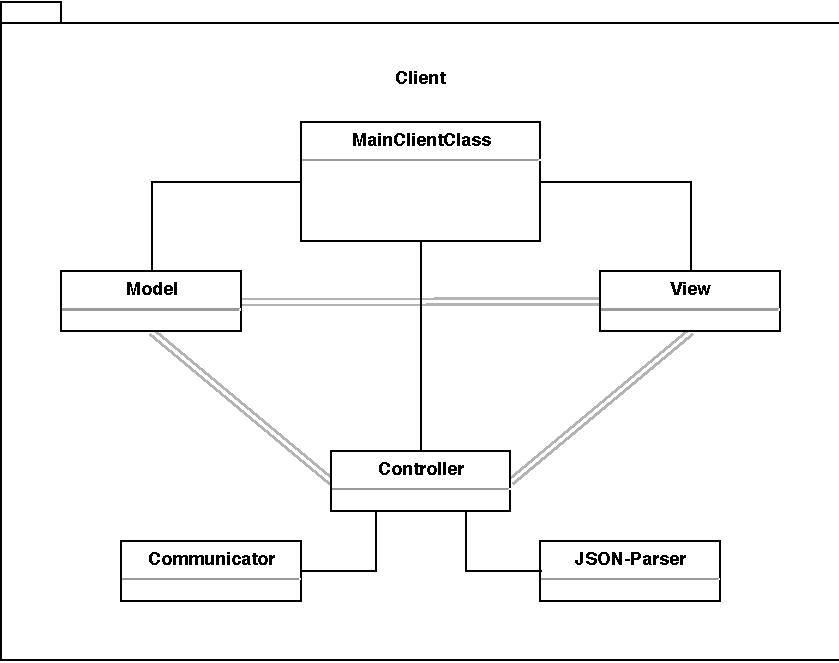
\includegraphics[scale=1]{images/Uebersicht.pdf}
    \end{figure}

\subsection{Beschreibung}
	Die Grundlegende Struktur der Client Anwendung basiert auf dem Model-View-Controller Modell (MVC Modell). Dabei werden alle Aufgaben weitestgehend auf drei unabhängige Klasse verteilt. In der Model Klasse sind alle für die Funktion der Anwendung benötigten Datenstrukturen enthalten. Die View Klasse ist dafür verantwortlich alle Daten in einer geeigneten Form darzustellen. Die Controller Klasse dient dazu, basierend auf verschiedenen Ereignissen, wie z.B. Benutzereingaben, die Daten im Model anzupassen, sodass in diesem Fall z.B. eine neue Spielsituation von der View abgebildet werden kann. Die Klassen Communicator und JSON-Parser stelle Hilfsklassen der Controller Klasse dar. 
		